\chapter{Chapter 2}
\label{Chp:2}
\section{A brief introduction to Machine Learning}
Machine Learning (ML) encompasses a broad set of methods that enable algorithms to learn complex patterns and relationships from data. While traditional approaches rely on manually engineering features, ML techniques automatically adjust their internal parameters to improve performance on a specific task. Here we specifically focus here on the application of Deep Learning, characterized by the utilization of Artificial Neural Networks (ANNs).

\begin{figure}[htbp]
    \centering
    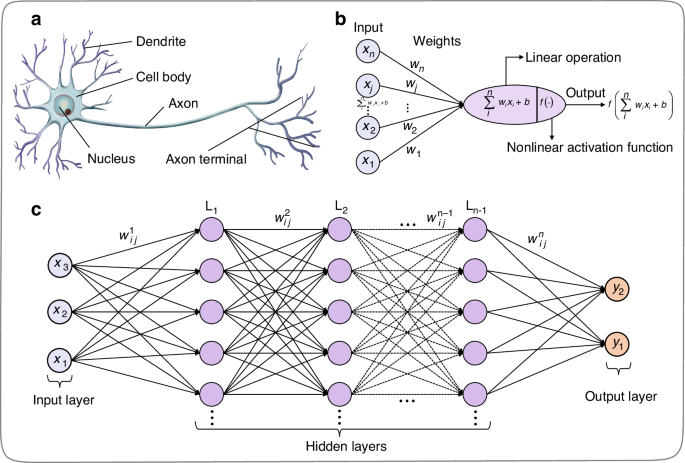
\includegraphics[width=0.95\textwidth]{img/ANN.png}
    \caption{Visual overview of neural networks. Panel a: A detailed illustration of a biological neuron with key structural components. Panel b: A schematic of an artificial neuron (Perceptron), demonstrating how weighted inputs are combined linearly and then passed through a non-linear activation function. Panel c: A Deep Neural Network, composed of stacked layers of artificial neurons, showing input, hidden, and output layers.}
    \label{fig:ann_overview}
\end{figure}

ANNs are computational models inspired by the structure and function of biological neural systems, which communicate via vast networks of neurons (fig.~\ref{fig:ann_overview}a). The fundamental computational unit is the artificial neuron (Fig.~\ref{fig:ann_overview}b). A single neuron computes a linear combination of its inputs $\mathbf{x}$ using a set of learnable weights $\mathbf{w}$ and a bias term $b$. This sum is then transformed by a non-linear activation function, $f(\cdot)$, which is essential for capturing complex, non-linear mappings.

By stacking these fundamental units into multiple layered structures, we create Deep Neural Networks (DNNs) (Fig.~\ref{fig:ann_overview}c). These architectures have proven highly effective in mapping high-dimensional function spaces and solving problems in diverse fields like computer vision, natural language processing, and physical modeling. A key theoretical foundation of ANNs is the \textit{Universal Approximation Theorem}. This theorem states that a feedforward network with a single hidden layer and a non-linear activation function can, in principle, approximate any continuous function on a compact set, given a sufficient number of neurons. First proven by Cybenko~\cite{cybenko1989approximation} and Hornik~\cite{hornik1989multilayer} in 1989, this principle highlights the fundamental expressive power of neural network architectures. Modern deep networks extend this concept by composing multiple non-linear transformations across numerous layers.


\section{Operator Learning}

Scientific Machine Learning (SciML) has emerged as a rapidly developing field that bridges the versatility of data-driven techniques—designed 
to recognize complex patterns from observations—with the rigor of traditional modeling based on partial differential equations (PDEs).

According to recent categorizations \cite{boulle2023mathematical}, the SciML landscape can be broadly divided into three main areas:
\begin{enumerate}
    \item \textbf{PDE Discovery}, which focuses on inverse problems to uncover governing equations from data;
    \item \textbf{Neural PDE Solvers}, which leverage neural networks to approximate the solution of specific PDE instances;
    \item \textbf{Operator Learning}, the most recent development, aimed at learning mappings between infinite-dimensional function spaces.
\end{enumerate}

The second area is related to direct problems and has proven effective in accelerating traditional solvers.
A revolution in this field was marked by the introduction of Physics-Informed Neural Networks (PINNs) and their variants \cite{raissi2019physics}. 
These architectures privilege a physics-oriented approach, embedding physical laws directly into the optimization process, rather than relying solely on data.
However, PINNs are typically trained to solve a \textit{single} problem instance efficiently. Since the solution depends on specific input parameters
or boundary conditions, changing these inputs often requires retraining the network, limiting their applicability in many-query scenarios.

To address this limitation, the third branch—\textbf{Operator Learning}—has been developed over the last few years \cite{lu2021learning, li2020fourier}.
 Unlike traditional solvers, operator learning algorithms aim to approximate the underlying operator itself, 
 mapping an entire class of input functions to their corresponding solutions. This approach has been successfully applied to complex PDE systems 
 involving parametric dependencies and forcing terms, as well as in industrial applications \cite{osorio2022forecasting}.

Among the emerging approaches, two architectures stand out: the Deep Operator Network (DeepONet) \cite{lu2021learning}, 
based on the universal approximation theorem for operators, and Neural Operators \cite{kovachki2023neural}. Specifically, 
integral kernel-based methods such as the Fourier Neural Operator (FNO) \cite{li2020fourier}
have demonstrated remarkable capabilities in learning non-linear operators on regular or equispaced domains.

\begin{figure}[htbp]
    \centering
    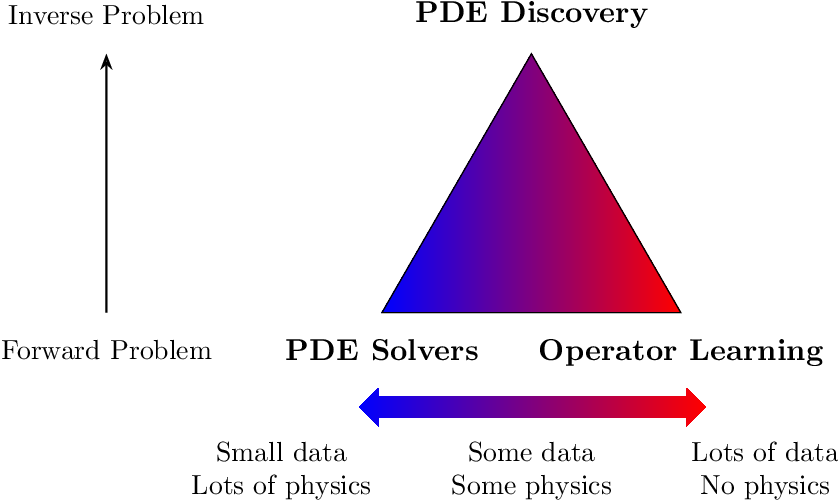
\includegraphics[width=0.75\textwidth]{img/Operator_learning.png}
    \caption{Visual representation of the Scientific Machine Learning (SciML) landscape.}
    \label{fig:sciml_landscape}
\end{figure}

\newpage

\subsection{Neural Architectures}
\subsubsection{Deep Operator Network (DeepONet)}
The DeepONet, introduced by Lu et al. \cite{lu2021learning}, was the first architecture explicitly designed as a concrete realization of the universal approximation theorem for operators by Chen and Chen \cite{Chen_Chen_1995}.
The architecture, schematized in Figure \ref{fig:deeponet_schema}, is composed of two distinct neural subnetworks working in parallel:
\begin{itemize}
    \item \textbf{Branch Network:} encodes the input function $f$ evaluated at a finite number of sensor points $x_1, \dots, x_m$.
    \item \textbf{Trunk Network:} encodes the domain coordinates $y$ where the solution is to be evaluated.
\end{itemize}
The output of the approximated operator is obtained through the dot product of the outputs of these two networks, allowing the solution to generalize across the entire continuous domain \cite{lu2021learning}:
\begin{equation}
    \hat{G}_{\theta}(f)(y) = \sum_{k=1}^{p} \underbrace{b_k(f(x_1), \dots, f(x_m))}_{\text{Branch Net}} \cdot \underbrace{t_k(y)}_{\text{Trunk Net}}
\end{equation}

\begin{figure}[H]
    \centering
    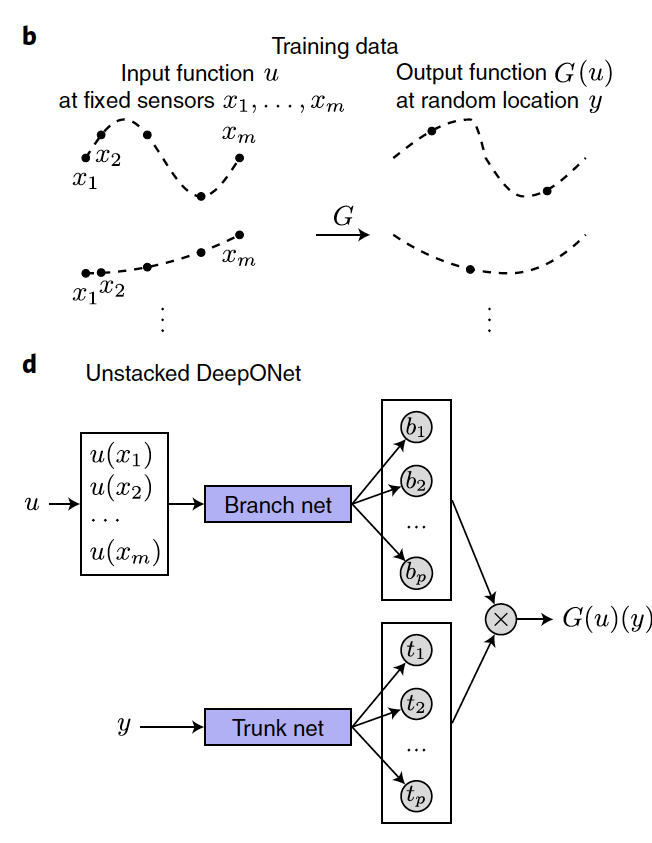
\includegraphics[width=0.8\textwidth]{img/FH_model/DeepONet.png}
    \caption{Schematic of the DeepONet architecture. The \textit{branch net} processes the discretized input function, while the \textit{trunk net} processes the domain coordinates. Their outputs are combined via a dot product. Adapted from \cite{lu2021learning}.}
    \label{fig:deeponet_schema}
\end{figure}

\subsubsection{Fourier Neural Operator (FNO)}
The Fourier Neural Operator (FNO), proposed by Li et al. \cite{li2020fourier}, tackles the approximation problem by parameterizing the integral operator directly in the frequency domain. Unlike standard networks, FNO learns a mapping between infinite-dimensional function spaces, guaranteeing discretization independence (\textit{resolution-invariance}).

As shown in Figure \ref{fig:fno_schema}, the architecture follows three main phases:
\begin{enumerate}
    \item \textbf{Lifting:} The input $a(x)$ is lifted to a higher-dimensional hidden representation $v_0(x)$ via a local transformation $P$ (typically a shallow fully connected network with activation $\sigma_1$): \\
    $v_0(x) = P(a(x)) = \sigma_1(W_{\text{in}} a(x) + b_{\text{in}}), \quad x \in D.$
    
    \item \textbf{Iterative Kernel Updates:} For $t = 0, \dots, T-1$, the hidden representation is updated using a pointwise linear operator $W_t$, an integral kernel operator with parameterized kernel $\kappa_t$, and the non-linear activation function $\sigma_2$: \\
    $\displaystyle v_{t+1}(x) = \sigma_2 \left( W_t v_t(x) + \int_{D} \kappa_t(x,y) v_t(y) \, dy + b_t \right).$
    
    \item \textbf{Projection:} The final hidden representation $v_T$ is projected back to the target space defined on $D'$ using another local transformation $Q$ (with activation $\sigma_3$): \\
    $\mathcal{G}(a)(x) = Q(v_T(x)) = \sigma_3(W_{\text{out}} v_T(x) + b_{\text{out}}), \quad x \in D'.$
\end{enumerate}

In the specific case of the Fourier Neural Operator (FNO) \cite{li2020fourier}, the integral kernel is parameterized directly in the frequency domain. By leveraging the convolution theorem, the continuous integral operation is efficiently resolved by computing the Fourier transform of the input, performing a pointwise multiplication with a learnable complex-valued weight tensor over a truncated set of low-frequency modes,
%Devo parlare della relazione che deve intercorrere tra le frequenze considerate $k_max$ ed il numero di campioni $N$ (Teorema di Nysquist-Shannon?)
 and finally applying the inverse Fourier transform. Mathematically, the integral term in the iterative update is replaced by:
\[ 
\int_{D} \kappa_t(x,y) v_t(y) \, dy = \mathcal{F}^{-1} \left( R_t \cdot \mathcal{F}(v_t) \right)(x) 
\]
where $\mathcal{F}$ and $\mathcal{F}^{-1}$ denote the forward and inverse Fourier transforms, respectively, and $R_t$ is the learnable complex tensor acting as the Fourier kernel at layer $t$. The truncation of higher frequencies acts as a low-pass filter, ensuring both discretization invariance and high computational efficiency.

\begin{figure}[H]
    \centering
    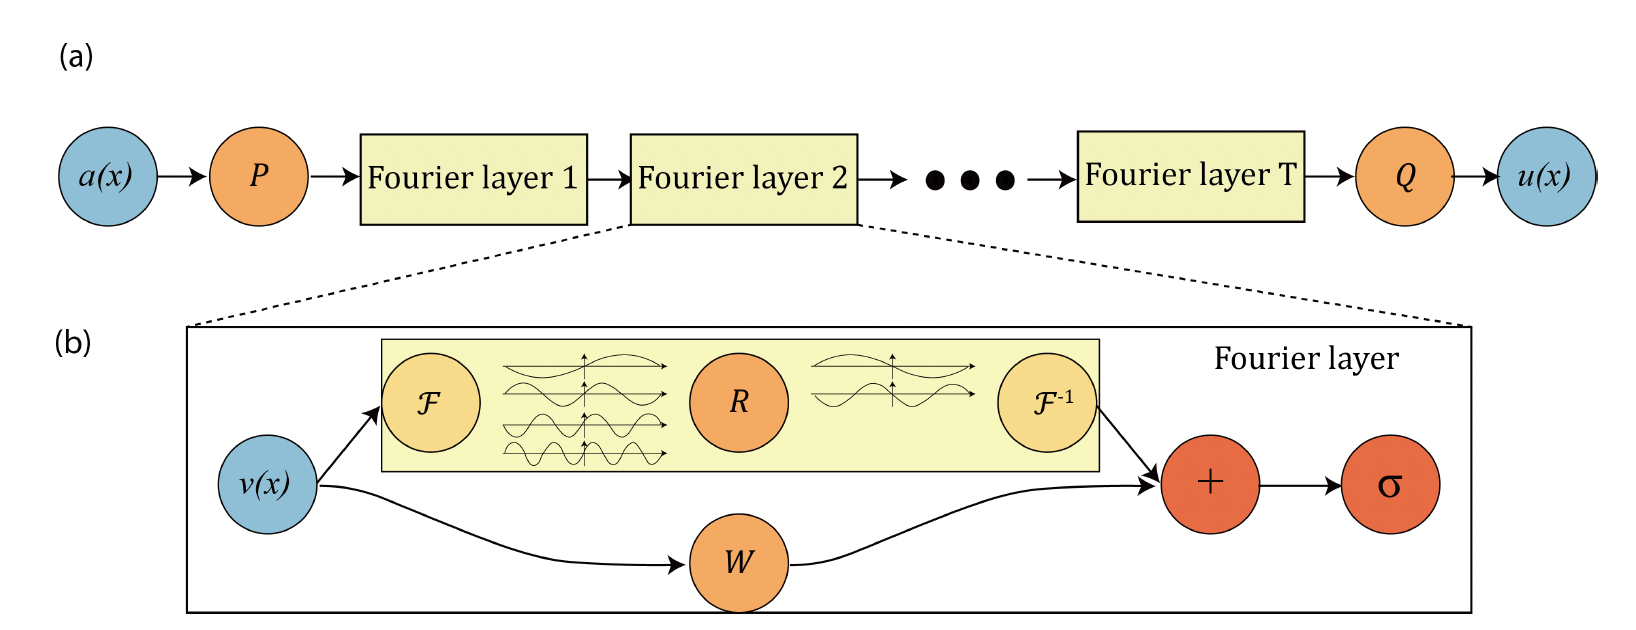
\includegraphics[width=\textwidth]{img/FH_model/FNO.png}
    \caption{Schematic of the FNO architecture. (a) General structure with lifting ($P$), iterative layers ($T$), and projection ($Q$). (b) Detail of a single Fourier layer. Adapted from \cite{li2020fourier}.}
    \label{fig:fno_schema}
\end{figure}

\newpage
\section{Approximation theorems}
\subsection{Universal approximation of functions}
To fully understand the universal approximation capabilities of Artificial Neural Networks, we first need to introduce the formal mathematical framework and notation established by Hornik, Stinchcombe, and White \cite{hornik1989multilayer}. 

Let $r \in \mathbb{N}$ be the dimension of the input space. We define $A^r$ as the set of all affine functions mapping $\mathbb{R}^r$ to $\mathbb{R}$:
$$ A^r = \{ A: \mathbb{R}^r \to \mathbb{R} \mid A(x) = w \cdot x + b, \; w, x \in \mathbb{R}^r, \; b \in \mathbb{R} \} $$
In a neural network context, $x$ represents the network input, $w$ the weights from the input to the intermediate layer, and $b$ the bias term.

A fundamental component of these architectures is the activation function, specifically a \textbf{squashing function}. A function $\Psi: \mathbb{R} \to [0, 1]$ is defined as a squashing function if it is \textit{non-decreasing}, $ \mathit{\lim_{\lambda \to \infty} \Psi(\lambda) = 1}$, and $\mathit{\lim_{\lambda \to -\infty} \Psi(\lambda) = 0}$.

Using these components, we define the class of output functions for a single hidden layer feedforward network. For any squashing function $\Psi$, the set $\Sigma^r(\Psi)$ is defined as:
$$ \Sigma^r(\Psi) = \left\{ f: \mathbb{R}^r \to \mathbb{R} \mathrel{\Big|} f(x) = \sum_{j=1}^q \beta_j \Psi(A_j(x)), \; \beta_j \in \mathbb{R}, \; A_j \in A^r, \; q \in \mathbb{N} \right\} $$
This represents the familiar class of output functions for networks with squashing at the hidden layer and a linear output layer, where the scalars $\beta_j$ correspond to the weights from the hidden to the output layer.

To rigorously evaluate how well these networks approximate other functions, we introduce the relevant mathematical spaces defined over the domain $\mathbb{R}^r$:
\begin{itemize}
    \item $\mathcal{B}^r$: The Borel $\sigma$-algebra on $\mathbb{R}^r$.
    \item $M^r$: The set of all Borel measurable functions $f: \mathbb{R}^r \to \mathbb{R}$.
    \item $C^r$: The set of all continuous functions $f: \mathbb{R}^r \to \mathbb{R}$ (note that $C^r \subset M^r$).
\end{itemize}

Finally, we define the approximation metrics:
\begin{itemize}
    \item \textbf{Uniformly dense on compacta:} A subset $S$ is uniformly dense on compacta in $C^r$ if, for every compact subset $K \subset \mathbb{R}^r$, $S$ is dense in $C^r$ with respect to the supremum metric $\rho_K(f, g) = \sup_{x \in K} |f(x) - g(x)|$.
    \item \textbf{$\rho_\mu$-dense:} Given a probability measure $\mu$ on $(\mathbb{R}^r, \mathcal{B}^r)$, which describes the relative frequency of occurrence of input patterns, we define the metric $\rho_\mu(f, g) = \inf\{\epsilon > 0 : \mu\{|f(x) - g(x)| > \epsilon\} < \epsilon\}$. Two functions are close in this metric if they differ significantly only on a set of inputs with a vanishingly small probability.
\end{itemize}

With this framework, we can state the fundamental approximation theorem for standard ANNs:

\begin{theorem}[Hornik, Stinchcombe, White, 1989]
For every squashing function $\Psi$, every $r$, and every probability measure $\mu$ on $(\mathbb{R}^r, \mathcal{B}^r)$, $\Sigma^r(\Psi)$ is uniformly dense on compacta in $C^r$ and $\rho_\mu$-dense in $M^r$.
\end{theorem}

%Il teorema generale è per più layers (almeno uno hidden). Lascio questa versione?

\subsection{Universal approximation of operators}

The universal approximation theorem by Hornik et al. guarantees that standard neural networks can approximate any continuous function between finite-dimensional spaces. However, many physical systems and partial differential equations (PDEs) require mapping an infinite-dimensional space to another infinite-dimensional space (e.g., mapping a parametric initialization or a boundary condition to a complete solution field over time). To address this, the operator learning paradigm extends the concept of universal approximation to operators.

The foundational theoretical work for operator approximation was established by Chen and Chen \cite{Chen_Chen_1995}, who demonstrated that a neural network with a specific architecture can approximate any continuous nonlinear operator. This theorem directly inspired the DeepONet architecture \cite{lu2021learning}.

Let $K_1 \subset \mathbb{R}^{d_1}$ and $K_2 \subset \mathbb{R}^{d_2}$ be compact sets. Let $V$ be a compact set in the space of continuous functions $C(K_1)$. We define a continuous nonlinear operator $\mathcal{G} : V \to C(K_2)$. 

\begin{theorem}[Universal Approximation Theorem for Operators, Chen \& Chen, 1995]
Suppose $\sigma$ is a continuous non-polynomial function. For any $\epsilon > 0$, there exist positive integers $n, m$, points $x_1, \dots, x_m \in K_1$, and constants $c_i, \xi_{ij}, \theta_i, \zeta_i \in \mathbb{R}$, $w_i \in \mathbb{R}^{d_2}$ (for $i=1,\dots,n$ and $j=1,\dots,m$) such that:
$$ \left| \mathcal{G}(u)(y) - \sum_{i=1}^n c_i \sigma \left( \sum_{j=1}^m \xi_{ij} u(x_j) + \theta_i \right) \sigma(w_i \cdot y + \zeta_i) \right| < \epsilon $$
holds for all $u \in V$ and $y \in K_2$.
\end{theorem}

This theorem explicitly reflects the dual-network structure of DeepONet. The term $\sigma\left(\sum_{j=1}^m \xi_{ij} u(x_j) + \theta_i\right)$ is parameterized by the \textit{branch net}, which takes discrete evaluations of the input function $u$ at sensor locations $x_j$. Conversely, the term $\sigma(w_i \cdot y + \zeta_i)$ is parameterized by the \textit{trunk net}, which evaluates the continuous spatial or temporal coordinates $y$.


\subsection{Universal approximation of operators II}

While the theorem by Chen and Chen \cite{Chen_Chen_1995} provides a fundamental result for continuous functions on compact sets, modern Scientific Machine Learning tasks often require learning operators under specific physical constraints, working with Lebesgue or Sobolev spaces, and minimizing the expected error over a specific probability measure of the initial conditions or parameters.

Kovachki et al. \cite{kovachki2023neural} provide a comprehensive approximation theory for Neural Operators, proving that an architecture based on alternating integral kernel operators and pointwise non-linearities is a universal approximator for operators between general Banach spaces. 

To formally state the theorems, we first need to define the function spaces for which these results hold.

\subsection{Function Space Assumptions}

The theory relies on the input and output spaces possessing the \textit{Banach Space Approximation Property (AP)}, which allows infinite-dimensional operators to be approximated by finite-rank operators. The authors restrict the analysis to the following widely used spaces.

\begin{assumption}[Input Space $\mathcal{A}$]
Let $D \subset \mathbb{R}^d$ be a Lipschitz domain. The input Banach space $\mathcal{A}$ satisfies one of the following:
\begin{enumerate}
    \item $\mathcal{A} = L^{p_1}(D)$ for some $1 \le p_1 < \infty$;
    \item $\mathcal{A} = W^{m_1,p_1}(D)$ for some $1 \le p_1 < \infty$ and $m_1 \in \mathbb{N}$;
    \item $\mathcal{A} = C(\overline{D})$.
\end{enumerate}
\end{assumption}

\begin{assumption}[Output Space $\mathcal{U}$]
Let $D' \subset \mathbb{R}^{d'}$ be a Lipschitz domain. The output Banach space $\mathcal{U}$ satisfies one of the following:
\begin{enumerate}
    \item $\mathcal{U} = L^{p_2}(D')$ for some $1 \le p_2 < \infty$ and $m_2 = 0$;
    \item $\mathcal{U} = W^{m_2,p_2}(D')$ for some $1 \le p_2 < \infty$ and $m_2 \in \mathbb{N}$;
    \item $\mathcal{U} = C^{m_2}(\overline{D}')$ with $m_2 \in \mathbb{N}_0$.
\end{enumerate}
\end{assumption}

The theoretical architecture of the Neural Operator, denoted as $NO_N(\sigma_1, \sigma_2, \sigma_3; D, D')$, represents the class of neural operators where $N \in \mathbb{N}$ is the number of integral layers (the depth of the network), $\sigma_1, \sigma_2, \sigma_3$ are the non-linear activation functions used respectively for the initial lifting mapping, the iterative kernel layers, and the final projection mapping, while $D$ and $D'$ are the input and output spatial domains. This architecture is specifically constructed so that its continuous layers can seamlessly approximate infinite-dimensional mappings with arbitrary precision. Note that for FNO $D=D'$.

\begin{theorem}[Uniform Universal Approximation, Kovachki et al. \cite{kovachki2023neural}]
Suppose the spaces $\mathcal{A}$ and $\mathcal{U}$ satisfy the aforementioned Assumptions and let $\mathcal{G}^{\dagger} : \mathcal{A} \to \mathcal{U}$ be a continuous operator. Let $\sigma_1, \sigma_2, \sigma_3$ be suitable non-polynomial continuous activation functions. 
Then, for any compact set $K \subset \mathcal{A}$ and any $\epsilon > 0$, there exists an integer $N \in \mathbb{N}$ and a Neural Operator $\mathcal{G} \in NO_N(\sigma_1, \sigma_2, \sigma_3; D, D')$ such that:
\[ 
\sup_{a \in K} \left\| \mathcal{G}^{\dagger}(a) - \mathcal{G}(a) \right\|_{\mathcal{U}} \le \epsilon 
\]
Furthermore, if $\mathcal{U}$ is a Hilbert space and there exists $M > 0$ such that $\|\mathcal{G}^{\dagger}(a)\|_{\mathcal{U}} \le M$ for all $a \in \mathcal{A}$, then $\mathcal{G}$ can be chosen such that uniformly $\|\mathcal{G}(a)\|_{\mathcal{U}} \le 4M$ for all $a \in \mathcal{A}$.
\end{theorem}

\newpage
\section{Discretization invariance and resolution independence}

A defining characteristic of Neural Operators, which distinguishes them from classical deep learning architectures such as Convolutional Neural Networks (CNNs), is the property of \textit{discretization invariance}. In standard architectures, model parameters are intrinsically tied to the specific discretization of the input data (e.g., the number of pixels in an image or the grid size of a simulation). Conversely, Neural Operators are defined as mappings between infinite-dimensional function spaces, meaning the learned parameters are independent of the underlying mesh used during training \cite{kovachki2023neural}.

\subsection{Intuition}

An operator learning architecture is said to be discretization-invariant if the model parameters $\theta$ are defined in a continuous function space and can be applied to any discretization of the input and output domains $D, D'$. 

Following Li et al. \cite{li2020fourier}, let $a \in \mathcal{A}$ be the input function. In a practical setting, we only observe $a$ at a finite set of points $\{x_1, \dots, x_n\} \subset D$. While a standard neural network would learn a mapping $\mathbb{R}^n \to \mathbb{R}^m$, the Neural Operator learns an operator $\mathcal{G}_{\theta}: \mathcal{A} \to \mathcal{U}$. The discretization $a_n$ of the function $a$ is used only to approximate the continuous integral:
\[ 
\int_{D} \kappa(x,y) v(y) \, dy \approx \sum_{j=1}^{n} \kappa(x, y_j) v(y_j) \Delta y_j 
\]
Because the kernel $\kappa$ (or its Fourier representation $R$ in FNOs) is a continuous object, the same parameters $\theta$ can be evaluated on a different set of points $\{x'_1, \dots, x'_k\}$ without retraining.

\subsection{Formal definition}

Since our data $a^{(i)}$ and $u^{(i)}$ are, in general, functions, to work with them numerically, we assume access only to their point-wise evaluations. To illustrate this, we will continue with the example of the preceding paragraph. For simplicity, assume $D = D'$ and suppose that the input and output functions are both real-valued. Let $D_L = \{x_{\ell}\}_{\ell=1}^L \subset D$ be an $L$-point discretization of the domain $D$ and assume we have observations $a^{(i)}|_{D_L}, u^{(i)}|_{D_L} \in \mathbb{R}^L$, for a finite collection of input-output pairs indexed by $i$. 

In the next section, we propose a kernel-inspired graph neural network architecture which, while trained on the discretized data, can produce the solution $u(x)$ for any $x \in D$ given an input $a \sim \mu$. In particular, our discretized architecture maps into the space $\mathcal{U}$ and not into a discretization thereof. Furthermore, our parametric operator class is consistent, in that, given a fixed set of parameters, refinement of the input discretization converges to the true function space operator. We make this notion precise in what follows and refer to architectures that possess it as \textit{function space architectures}, \textit{mesh-invariant architectures}, or \textit{discretization-invariant architectures}.

\begin{definition}[Discrete refinement]
We call a discrete refinement of the domain $D \subset \mathbb{R}^d$ any sequence of nested sets $D_1 \subset D_2 \subset \dots \subset D$ with $|D_L| = L$ for any $L \in \mathbb{N}$ such that, for any $\epsilon > 0$, there exists a number $L = L(\epsilon) \in \mathbb{N}$ such that
\[
D \subseteq \bigcup_{x \in D_L} \{y \in \mathbb{R}^d : \|y - x\|_2 < \epsilon\}.
\]
\end{definition}

\begin{definition}[Discretization]
Given a discrete refinement $(D_L)_{L=1}^{\infty}$ of the domain $D \subset \mathbb{R}^d$, any member $D_L$ is called a discretization of $D$.
\end{definition}

Since $a : D \subset \mathbb{R}^d \to \mathbb{R}^m$, pointwise evaluation of the function (discretization) at a set of $L$ points gives rise to the data set $\{(x_{\ell}, a(x_{\ell}))\}_{\ell=1}^L$. Note that this may be viewed as a vector in $\mathbb{R}^{L \times d} \times \mathbb{R}^{L \times m}$.

\begin{definition}[Discretized uniform risk]
Suppose $\mathcal{A}$ is a Banach space of $\mathbb{R}^m$-valued functions on the domain $D \subset \mathbb{R}^d$. Let $G : \mathcal{A} \to \mathcal{U}$ be an operator, $D_L$ be an $L$-point discretization of $D$, and $\hat{G} : \mathbb{R}^{L \times d} \times \mathbb{R}^{L \times m} \to \mathcal{U}$ some map. For any $K \subset \mathcal{A}$ compact, we define the discretized uniform risk as:
\[
R_K(G, \hat{G}, D_L) = \sup_{a \in K} \| \hat{G}(D_L, a|_{D_L}) - G(a) \|_{\mathcal{U}}.
\]
\end{definition}

\begin{definition}[Discretization-invariant]
Let $\Theta \subseteq \mathbb{R}^p$ be a finite dimensional parameter space and $G : \mathcal{A} \times \Theta \to \mathcal{U}$ a map representing a parametric class of operators with parameters $\theta \in \Theta$. Given a discrete refinement $(D_n)_{n=1}^{\infty}$ of the domain $D \subset \mathbb{R}^d$, we say $G$ is discretization-invariant if there exists a sequence of maps $\hat{G}_1, \hat{G}_2, \dots$ where $\hat{G}_L : \mathbb{R}^{L \times d} \times \mathbb{R}^{L \times m} \times \Theta \to \mathcal{U}$ such that, for any $\theta \in \Theta$ and any compact set $K \subset \mathcal{A}$,
\[
\lim_{L \to \infty} R_K(G(\cdot, \theta), \hat{G}_L(\cdot, \cdot, \theta), D_L) = 0.
\]
\end{definition}

Such a property is highly desirable as it allows a transfer of solutions between different grid geometries and discretization sizes with a single architecture that has a fixed number of parameters. From the construction of neural operators, when the input and output functions are evaluated on fixed grids, the architecture of neural operators on these fixed grids coincide with the class of neural networks.

\subsection{Zero-Shot Super-Resolution}

The immediate consequence of discretization invariance is the ability to perform \textit{zero-shot super-resolution}. The neural operator is mesh-invariant, so it can be trained on a lower resolution and evaluated at a
higher resolution, without seeing any higher resolution data. 

As demonstrated in the numerical experiments for parametric PDEs \cite{li2020fourier}, the error of a discretization-invariant model remains consistent across different resolutions. This is formally expressed by the property that as the discretization becomes finer ($n \to \infty$), the discrete approximation converges to the continuous operator:
\[ 
\lim_{n \to \infty} \mathcal{G}_{\theta}(a_n) = \mathcal{G}_{\theta}(a) 
\]
This feature is particularly valuable in neuroscience and complex systems modeling, where neural field dynamics or networked ODEs may be simulated at different spatial scales. A Neural Operator trained on a low-resolution brain atlas or a small neural network can, in principle, generalize its learned dynamics to higher-resolution representations or larger networks without requiring new training data.


